\documentclass[border=3pt]{standalone}
% Preâmbulo compartilhado pelos diagramas TikZ da aula 7 de Navegação (Implementação do A*)
\usepackage[T1]{fontenc}
\usepackage[utf8]{inputenc}
\usepackage{lmodern}
\usepackage{amsmath}
\usepackage{xcolor}
\usepackage{tikz}
\usetikzlibrary{arrows.meta,angles,quotes,decorations.pathmorphing,decorations.pathreplacing,calc,
                positioning,shapes.geometric,shapes.misc,backgrounds,fit,
                math}

% Paleta (mesma dos SVGs originais)
\definecolor{dblue}{HTML}{2A5B8C}
\definecolor{dorange}{HTML}{B3541E}
\definecolor{dgreen}{HTML}{4A7C59}
\definecolor{dred}{HTML}{9C4B4B}
\definecolor{dcream}{HTML}{F4F1EA}
\definecolor{dshade}{HTML}{DDD7C9}

% Função gaussiana (não normalizada por padrão de escala visual)
\pgfmathdeclarefunction{gauss}{3}{%
  \pgfmathparse{1/(#3*sqrt(2*pi))*exp(-((#1-#2)^2)/(2*#3^2))}%
}

% Estilos comuns (prefixo d... para não colidir com chaves internas do pgf)
\tikzset{
  >={Stealth[length=2mm]},
  dguide/.style={gray!55, dashed, line width=0.4pt},
  daxis/.style={gray!60, line width=0.7pt, ->},
  dbody/.style={fill=black!3, draw=black!80, line width=1pt},
  dacc/.style={draw=dblue, line width=1pt},
  dlbl/.style={black!55, font=\small},
  dsub/.style={black!45, font=\footnotesize},
  dstate/.style={circle, draw=black!80, fill=dcream, line width=1pt,
                 minimum size=17mm, font=\large, inner sep=1pt},
  dobs/.style={circle, draw=black!80, fill=dshade, line width=1pt,
               minimum size=14mm, font=\large, inner sep=1pt},
  dbox/.style={rounded corners=2pt, draw=black!80, fill=dcream, line width=1pt,
               align=center, inner sep=6pt},
  dop/.style={circle, draw=black!80, fill=white, line width=1pt,
              minimum size=6mm, inner sep=0pt, font=\small},
  dtrans/.style={->, dblue, line width=1pt},
  dmeas/.style={->, dorange, line width=1pt},
  dcurve/.style={line width=1pt, dblue},
  dcurveb/.style={line width=1.4pt, dorange},
}

\begin{document}
\hyphenpenalty=10000 \exhyphenpenalty=10000 \tolerance=9999 \emergencystretch=3em
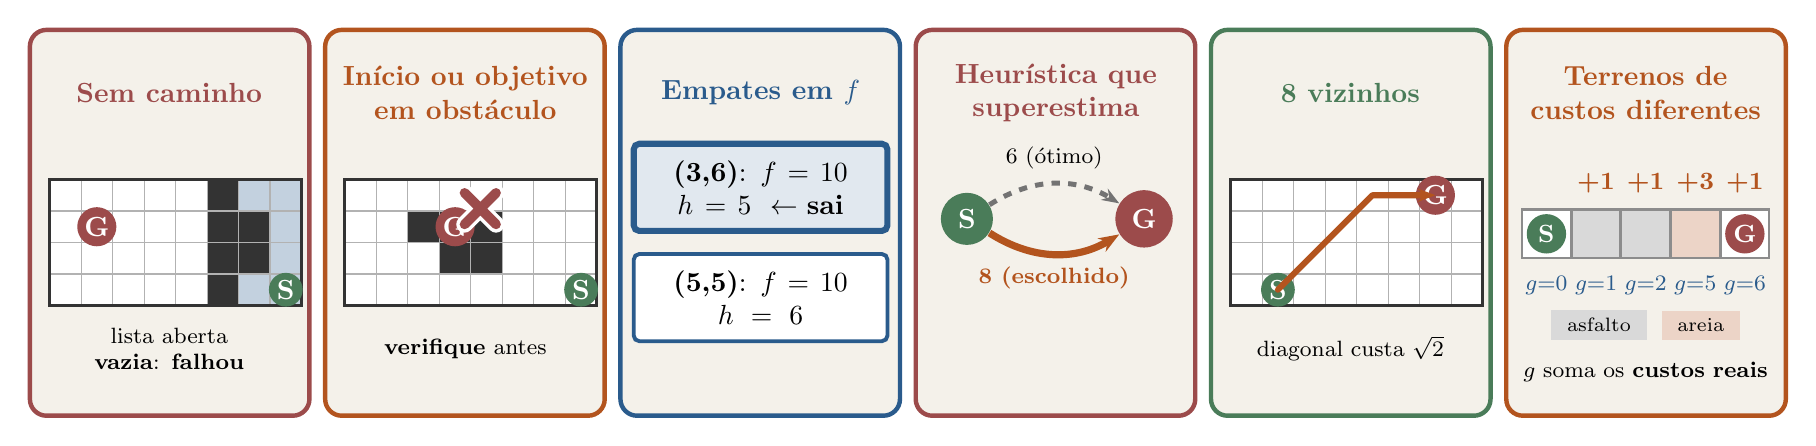
\begin{tikzpicture}[x=1cm,y=1cm]
\draw[dred, line width=1.6pt, rounded corners=6pt, fill=dcream] (0.00,0) rectangle (3.55,4.90);
\node[font=\normalsize\bfseries, dred, text width=3.2cm, align=center] at (1.77,4.10) {Sem caminho};
\draw[fill=white, draw=black!30, line width=0.4pt] (0.250,2.600) rectangle ++(0.400,0.400);
\draw[fill=white, draw=black!30, line width=0.4pt] (0.650,2.600) rectangle ++(0.400,0.400);
\draw[fill=white, draw=black!30, line width=0.4pt] (1.050,2.600) rectangle ++(0.400,0.400);
\draw[fill=white, draw=black!30, line width=0.4pt] (1.450,2.600) rectangle ++(0.400,0.400);
\draw[fill=white, draw=black!30, line width=0.4pt] (1.850,2.600) rectangle ++(0.400,0.400);
\draw[fill=black!80, draw=black!30, line width=0.4pt] (2.250,2.600) rectangle ++(0.400,0.400);
\draw[fill=dblue!28!white, draw=black!30, line width=0.4pt] (2.650,2.600) rectangle ++(0.400,0.400);
\draw[fill=dblue!28!white, draw=black!30, line width=0.4pt] (3.050,2.600) rectangle ++(0.400,0.400);
\draw[fill=white, draw=black!30, line width=0.4pt] (0.250,2.200) rectangle ++(0.400,0.400);
\draw[fill=white, draw=black!30, line width=0.4pt] (0.650,2.200) rectangle ++(0.400,0.400);
\draw[fill=white, draw=black!30, line width=0.4pt] (1.050,2.200) rectangle ++(0.400,0.400);
\draw[fill=white, draw=black!30, line width=0.4pt] (1.450,2.200) rectangle ++(0.400,0.400);
\draw[fill=white, draw=black!30, line width=0.4pt] (1.850,2.200) rectangle ++(0.400,0.400);
\draw[fill=black!80, draw=black!30, line width=0.4pt] (2.250,2.200) rectangle ++(0.400,0.400);
\draw[fill=black!80, draw=black!30, line width=0.4pt] (2.650,2.200) rectangle ++(0.400,0.400);
\draw[fill=dblue!28!white, draw=black!30, line width=0.4pt] (3.050,2.200) rectangle ++(0.400,0.400);
\draw[fill=white, draw=black!30, line width=0.4pt] (0.250,1.800) rectangle ++(0.400,0.400);
\draw[fill=white, draw=black!30, line width=0.4pt] (0.650,1.800) rectangle ++(0.400,0.400);
\draw[fill=white, draw=black!30, line width=0.4pt] (1.050,1.800) rectangle ++(0.400,0.400);
\draw[fill=white, draw=black!30, line width=0.4pt] (1.450,1.800) rectangle ++(0.400,0.400);
\draw[fill=white, draw=black!30, line width=0.4pt] (1.850,1.800) rectangle ++(0.400,0.400);
\draw[fill=black!80, draw=black!30, line width=0.4pt] (2.250,1.800) rectangle ++(0.400,0.400);
\draw[fill=black!80, draw=black!30, line width=0.4pt] (2.650,1.800) rectangle ++(0.400,0.400);
\draw[fill=dblue!28!white, draw=black!30, line width=0.4pt] (3.050,1.800) rectangle ++(0.400,0.400);
\draw[fill=white, draw=black!30, line width=0.4pt] (0.250,1.400) rectangle ++(0.400,0.400);
\draw[fill=white, draw=black!30, line width=0.4pt] (0.650,1.400) rectangle ++(0.400,0.400);
\draw[fill=white, draw=black!30, line width=0.4pt] (1.050,1.400) rectangle ++(0.400,0.400);
\draw[fill=white, draw=black!30, line width=0.4pt] (1.450,1.400) rectangle ++(0.400,0.400);
\draw[fill=white, draw=black!30, line width=0.4pt] (1.850,1.400) rectangle ++(0.400,0.400);
\draw[fill=black!80, draw=black!30, line width=0.4pt] (2.250,1.400) rectangle ++(0.400,0.400);
\draw[fill=dblue!28!white, draw=black!30, line width=0.4pt] (2.650,1.400) rectangle ++(0.400,0.400);
\draw[fill=dblue!28!white, draw=black!30, line width=0.4pt] (3.050,1.400) rectangle ++(0.400,0.400);
\draw[black!80, line width=1pt] (0.250,1.400) rectangle (3.450,3.000);
\node[circle, fill=dred, text=white, font=\bfseries\normalsize, inner sep=1pt, minimum size=0.32cm] at (0.850,2.400) {G};
\node[circle, fill=dgreen, text=white, font=\bfseries\normalsize, inner sep=1pt, minimum size=0.32cm] at (3.250,1.600) {S};
\node[font=\footnotesize, text width=3.2cm, align=center] at (1.77,0.85) {lista aberta \textbf{vazia}: \textbf{falhou}};
\draw[dorange, line width=1.6pt, rounded corners=6pt, fill=dcream] (3.75,0) rectangle (7.30,4.90);
\node[font=\normalsize\bfseries, dorange, text width=3.2cm, align=center] at (5.53,4.10) {Início ou objetivo em obstáculo};
\draw[fill=white, draw=black!30, line width=0.4pt] (4.000,2.600) rectangle ++(0.400,0.400);
\draw[fill=white, draw=black!30, line width=0.4pt] (4.400,2.600) rectangle ++(0.400,0.400);
\draw[fill=white, draw=black!30, line width=0.4pt] (4.800,2.600) rectangle ++(0.400,0.400);
\draw[fill=white, draw=black!30, line width=0.4pt] (5.200,2.600) rectangle ++(0.400,0.400);
\draw[fill=white, draw=black!30, line width=0.4pt] (5.600,2.600) rectangle ++(0.400,0.400);
\draw[fill=white, draw=black!30, line width=0.4pt] (6.000,2.600) rectangle ++(0.400,0.400);
\draw[fill=white, draw=black!30, line width=0.4pt] (6.400,2.600) rectangle ++(0.400,0.400);
\draw[fill=white, draw=black!30, line width=0.4pt] (6.800,2.600) rectangle ++(0.400,0.400);
\draw[fill=white, draw=black!30, line width=0.4pt] (4.000,2.200) rectangle ++(0.400,0.400);
\draw[fill=white, draw=black!30, line width=0.4pt] (4.400,2.200) rectangle ++(0.400,0.400);
\draw[fill=black!80, draw=black!30, line width=0.4pt] (4.800,2.200) rectangle ++(0.400,0.400);
\draw[fill=black!80, draw=black!30, line width=0.4pt] (5.200,2.200) rectangle ++(0.400,0.400);
\draw[fill=black!80, draw=black!30, line width=0.4pt] (5.600,2.200) rectangle ++(0.400,0.400);
\draw[fill=white, draw=black!30, line width=0.4pt] (6.000,2.200) rectangle ++(0.400,0.400);
\draw[fill=white, draw=black!30, line width=0.4pt] (6.400,2.200) rectangle ++(0.400,0.400);
\draw[fill=white, draw=black!30, line width=0.4pt] (6.800,2.200) rectangle ++(0.400,0.400);
\draw[fill=white, draw=black!30, line width=0.4pt] (4.000,1.800) rectangle ++(0.400,0.400);
\draw[fill=white, draw=black!30, line width=0.4pt] (4.400,1.800) rectangle ++(0.400,0.400);
\draw[fill=white, draw=black!30, line width=0.4pt] (4.800,1.800) rectangle ++(0.400,0.400);
\draw[fill=black!80, draw=black!30, line width=0.4pt] (5.200,1.800) rectangle ++(0.400,0.400);
\draw[fill=black!80, draw=black!30, line width=0.4pt] (5.600,1.800) rectangle ++(0.400,0.400);
\draw[fill=white, draw=black!30, line width=0.4pt] (6.000,1.800) rectangle ++(0.400,0.400);
\draw[fill=white, draw=black!30, line width=0.4pt] (6.400,1.800) rectangle ++(0.400,0.400);
\draw[fill=white, draw=black!30, line width=0.4pt] (6.800,1.800) rectangle ++(0.400,0.400);
\draw[fill=white, draw=black!30, line width=0.4pt] (4.000,1.400) rectangle ++(0.400,0.400);
\draw[fill=white, draw=black!30, line width=0.4pt] (4.400,1.400) rectangle ++(0.400,0.400);
\draw[fill=white, draw=black!30, line width=0.4pt] (4.800,1.400) rectangle ++(0.400,0.400);
\draw[fill=white, draw=black!30, line width=0.4pt] (5.200,1.400) rectangle ++(0.400,0.400);
\draw[fill=white, draw=black!30, line width=0.4pt] (5.600,1.400) rectangle ++(0.400,0.400);
\draw[fill=white, draw=black!30, line width=0.4pt] (6.000,1.400) rectangle ++(0.400,0.400);
\draw[fill=white, draw=black!30, line width=0.4pt] (6.400,1.400) rectangle ++(0.400,0.400);
\draw[fill=white, draw=black!30, line width=0.4pt] (6.800,1.400) rectangle ++(0.400,0.400);
\draw[black!80, line width=1pt] (4.000,1.400) rectangle (7.200,3.000);
\node[circle, fill=dred, text=white, font=\bfseries\normalsize, inner sep=1pt, minimum size=0.32cm] at (5.400,2.400) {G};
\node[circle, fill=dgreen, text=white, font=\bfseries\normalsize, inner sep=1pt, minimum size=0.32cm] at (7.000,1.600) {S};
\draw[white, line width=6pt, line cap=round] (5.520,2.430) -- ++(0.4,0.4) (5.520,2.830) -- ++(0.4,-0.4);
\draw[dred, line width=3.5pt, line cap=round] (5.520,2.430) -- ++(0.4,0.4) (5.520,2.830) -- ++(0.4,-0.4);
\node[font=\footnotesize, text width=3.2cm, align=center] at (5.53,0.85) {\textbf{verifique} antes};
\draw[dblue, line width=1.6pt, rounded corners=6pt, fill=dcream] (7.50,0) rectangle (11.05,4.90);
\node[font=\normalsize\bfseries, dblue, text width=3.2cm, align=center] at (9.28,4.10) {Empates em $f$};
\node[dbox, draw=dblue, fill=dblue!14, line width=2.2pt, text width=2.8cm, minimum height=1.1cm, font=\normalsize] at (9.28,2.9) {\textbf{(3,6)}: $f=10$\\ $h=5$ \ $\leftarrow$ \textbf{sai}};
\node[dbox, draw=dblue, fill=white, line width=1.4pt, text width=2.8cm, minimum height=1.1cm, font=\normalsize] at (9.28,1.5) {\textbf{(5,5)}: $f=10$\\ $h=6$};
\draw[dred, line width=1.6pt, rounded corners=6pt, fill=dcream] (11.25,0) rectangle (14.80,4.90);
\node[font=\normalsize\bfseries, dred, text width=3.2cm, align=center] at (13.03,4.10) {Heurística que superestima};
\node[circle, fill=dgreen, text=white, font=\bfseries\normalsize, minimum size=0.65cm] (sa) at (11.90,2.5) {S};
\node[circle, fill=dred, text=white, font=\bfseries\normalsize, minimum size=0.65cm] (ga) at (14.15,2.5) {G};
\draw[black!55, dashed, line width=1.8pt, -{Stealth[length=2.2mm]}] (sa) to[bend left=32] node[above, font=\footnotesize, black, pos=0.5, yshift=1pt] {6 (ótimo)} (ga);
\draw[dorange, line width=2.6pt, -{Stealth[length=2.6mm]}] (sa) to[bend right=32] node[below, font=\footnotesize\bfseries, dorange, pos=0.5] {8 (escolhido)} (ga);
\draw[dgreen, line width=1.6pt, rounded corners=6pt, fill=dcream] (15.00,0) rectangle (18.55,4.90);
\node[font=\normalsize\bfseries, dgreen, text width=3.2cm, align=center] at (16.77,4.10) {8 vizinhos};
\draw[fill=white, draw=black!30, line width=0.4pt] (15.250,2.600) rectangle ++(0.400,0.400);
\draw[fill=white, draw=black!30, line width=0.4pt] (15.650,2.600) rectangle ++(0.400,0.400);
\draw[fill=white, draw=black!30, line width=0.4pt] (16.050,2.600) rectangle ++(0.400,0.400);
\draw[fill=white, draw=black!30, line width=0.4pt] (16.450,2.600) rectangle ++(0.400,0.400);
\draw[fill=white, draw=black!30, line width=0.4pt] (16.850,2.600) rectangle ++(0.400,0.400);
\draw[fill=white, draw=black!30, line width=0.4pt] (17.250,2.600) rectangle ++(0.400,0.400);
\draw[fill=white, draw=black!30, line width=0.4pt] (17.650,2.600) rectangle ++(0.400,0.400);
\draw[fill=white, draw=black!30, line width=0.4pt] (18.050,2.600) rectangle ++(0.400,0.400);
\draw[fill=white, draw=black!30, line width=0.4pt] (15.250,2.200) rectangle ++(0.400,0.400);
\draw[fill=white, draw=black!30, line width=0.4pt] (15.650,2.200) rectangle ++(0.400,0.400);
\draw[fill=white, draw=black!30, line width=0.4pt] (16.050,2.200) rectangle ++(0.400,0.400);
\draw[fill=white, draw=black!30, line width=0.4pt] (16.450,2.200) rectangle ++(0.400,0.400);
\draw[fill=white, draw=black!30, line width=0.4pt] (16.850,2.200) rectangle ++(0.400,0.400);
\draw[fill=white, draw=black!30, line width=0.4pt] (17.250,2.200) rectangle ++(0.400,0.400);
\draw[fill=white, draw=black!30, line width=0.4pt] (17.650,2.200) rectangle ++(0.400,0.400);
\draw[fill=white, draw=black!30, line width=0.4pt] (18.050,2.200) rectangle ++(0.400,0.400);
\draw[fill=white, draw=black!30, line width=0.4pt] (15.250,1.800) rectangle ++(0.400,0.400);
\draw[fill=white, draw=black!30, line width=0.4pt] (15.650,1.800) rectangle ++(0.400,0.400);
\draw[fill=white, draw=black!30, line width=0.4pt] (16.050,1.800) rectangle ++(0.400,0.400);
\draw[fill=white, draw=black!30, line width=0.4pt] (16.450,1.800) rectangle ++(0.400,0.400);
\draw[fill=white, draw=black!30, line width=0.4pt] (16.850,1.800) rectangle ++(0.400,0.400);
\draw[fill=white, draw=black!30, line width=0.4pt] (17.250,1.800) rectangle ++(0.400,0.400);
\draw[fill=white, draw=black!30, line width=0.4pt] (17.650,1.800) rectangle ++(0.400,0.400);
\draw[fill=white, draw=black!30, line width=0.4pt] (18.050,1.800) rectangle ++(0.400,0.400);
\draw[fill=white, draw=black!30, line width=0.4pt] (15.250,1.400) rectangle ++(0.400,0.400);
\draw[fill=white, draw=black!30, line width=0.4pt] (15.650,1.400) rectangle ++(0.400,0.400);
\draw[fill=white, draw=black!30, line width=0.4pt] (16.050,1.400) rectangle ++(0.400,0.400);
\draw[fill=white, draw=black!30, line width=0.4pt] (16.450,1.400) rectangle ++(0.400,0.400);
\draw[fill=white, draw=black!30, line width=0.4pt] (16.850,1.400) rectangle ++(0.400,0.400);
\draw[fill=white, draw=black!30, line width=0.4pt] (17.250,1.400) rectangle ++(0.400,0.400);
\draw[fill=white, draw=black!30, line width=0.4pt] (17.650,1.400) rectangle ++(0.400,0.400);
\draw[fill=white, draw=black!30, line width=0.4pt] (18.050,1.400) rectangle ++(0.400,0.400);
\draw[black!80, line width=1pt] (15.250,1.400) rectangle (18.450,3.000);
\node[circle, fill=dgreen, text=white, font=\bfseries\normalsize, inner sep=1pt, minimum size=0.32cm] at (15.850,1.600) {S};
\node[circle, fill=dred, text=white, font=\bfseries\normalsize, inner sep=1pt, minimum size=0.32cm] at (17.850,2.800) {G};
\draw[dorange, line width=2.2pt, line cap=round, line join=round, -{Stealth[length=2.2mm]}] (15.850,1.600) -- (16.250,2.000) -- (16.650,2.400) -- (17.050,2.800) -- (17.450,2.800) -- (17.850,2.800);
\node[font=\footnotesize, text width=3.2cm, align=center] at (16.77,0.85) {diagonal custa $\sqrt{2}$};
\draw[dorange, line width=1.6pt, rounded corners=6pt, fill=dcream] (18.75,0) rectangle (22.30,4.90);
\node[font=\normalsize\bfseries, dorange, text width=3.2cm, align=center] at (20.52,4.10) {Terrenos de custos diferentes};
\draw[fill=white, draw=black!45, line width=0.8pt] (18.95,2.0) rectangle ++(0.62,0.62);
\node[circle, fill=dgreen, text=white, font=\bfseries\small, minimum size=0.5cm, inner sep=0.5pt] at (19.26,2.31) {S};
\node[font=\small\bfseries, dorange] at (19.26,2.95) {};
\node[font=\footnotesize, dblue] at (19.26,1.65) {$g{=}0$};
\draw[fill=black!15, draw=black!45, line width=0.8pt] (19.58,2.0) rectangle ++(0.62,0.62);
\node[font=\small\bfseries, dorange] at (19.89,2.95) {+1};
\node[font=\footnotesize, dblue] at (19.89,1.65) {$g{=}1$};
\draw[fill=black!15, draw=black!45, line width=0.8pt] (20.21,2.0) rectangle ++(0.62,0.62);
\node[font=\small\bfseries, dorange] at (20.52,2.95) {+1};
\node[font=\footnotesize, dblue] at (20.52,1.65) {$g{=}2$};
\draw[fill=dorange!25!white, draw=black!45, line width=0.8pt] (20.84,2.0) rectangle ++(0.62,0.62);
\node[font=\small\bfseries, dorange] at (21.15,2.95) {+3};
\node[font=\footnotesize, dblue] at (21.15,1.65) {$g{=}5$};
\draw[fill=white, draw=black!45, line width=0.8pt] (21.47,2.0) rectangle ++(0.62,0.62);
\node[circle, fill=dred, text=white, font=\bfseries\small, minimum size=0.5cm, inner sep=0.5pt] at (21.78,2.31) {G};
\node[font=\small\bfseries, dorange] at (21.78,2.95) {+1};
\node[font=\footnotesize, dblue] at (21.78,1.65) {$g{=}6$};
\node[font=\scriptsize] at (20.52,1.15) {\colorbox{black!15}{ asfalto } \ \colorbox{dorange!25!white}{ areia }};
\node[font=\footnotesize, text width=3.2cm, align=center] at (20.52,0.55) {$g$ soma os \textbf{custos reais}};
\end{tikzpicture}
\end{document}
